%============================================================================%
%
%	DOCUMENT DEFINITION
%
%============================================================================%

\documentclass[10pt,A4,english]{article}	


%----------------------------------------------------------------------------------------
%	ENCODING
%----------------------------------------------------------------------------------------

% we use utf8 since we want to build from any machine
\usepackage[utf8]{inputenc}		
\usepackage[USenglish]{isodate}
\usepackage{fancyhdr}
\usepackage[numbers]{natbib}

%----------------------------------------------------------------------------------------
%	LOGIC
%----------------------------------------------------------------------------------------

% provides \isempty test
\usepackage{xstring, xifthen}
\usepackage{enumitem}
\usepackage[english]{babel}
\usepackage{blindtext}
\usepackage{pdfpages}
\usepackage{changepage}
%----------------------------------------------------------------------------------------
%	FONT BASICS
%----------------------------------------------------------------------------------------

% some tex-live fonts - choose your own

%\usepackage[defaultsans]{droidsans}
%\usepackage[default]{comfortaa}
%\usepackage{cmbright}
\usepackage[default]{raleway}
%\usepackage{fetamont}
%\usepackage[default]{gillius}
%\usepackage[light,math]{iwona}
%\usepackage[thin]{roboto} 

% set font default
\renewcommand*\familydefault{\sfdefault} 	
\usepackage[T1]{fontenc}

% more font size definitions
\usepackage{moresize}

%----------------------------------------------------------------------------------------
%	FONT AWESOME ICONS
%---------------------------------------------------------------------------------------- 

% include the fontawesome icon set
\usepackage{fontawesome}

% use to vertically center content
% credits to: http://tex.stackexchange.com/questions/7219/how-to-vertically-center-two-images-next-to-each-other
\newcommand{\vcenteredinclude}[1]{\begingroup
\setbox0=\hbox{\includegraphics{#1}}%
\parbox{\wd0}{\box0}\endgroup}
\newcommand{\tab}[1]{\hspace{.2\textwidth}\rlap{#1}}
% use to vertically center content
% credits to: http://tex.stackexchange.com/questions/7219/how-to-vertically-center-two-images-next-to-each-other
\newcommand*{\vcenteredhbox}[1]{\begingroup
\setbox0=\hbox{#1}\parbox{\wd0}{\box0}\endgroup}

% icon shortcut
\newcommand{\icon}[3] { 							
	\makebox(#2, #2){\textcolor{maincol}{\csname fa#1\endcsname}}
}	


% icon with text shortcut
\newcommand{\icontext}[4]{ 						
	\vcenteredhbox{\icon{#1}{#2}{#3}}  \hspace{2pt}  \parbox{0.9\mpwidth}{\textcolor{#4}{#3}}
}

% icon with website url
\newcommand{\iconhref}[5]{ 						
    \vcenteredhbox{\icon{#1}{#2}{#5}}  \hspace{2pt} \href{#4}{\textcolor{#5}{#3}}
}

% icon with email link
\newcommand{\iconemail}[5]{ 						
    \vcenteredhbox{\icon{#1}{#2}{#5}}  \hspace{2pt} \href{mailto:#4}{\textcolor{#5}{#3}}
}

%----------------------------------------------------------------------------------------
%	PAGE LAYOUT  DEFINITIONS
%----------------------------------------------------------------------------------------

% page outer frames (debug-only)
% \usepackage{showframe}		

% we use paracol to display breakable two columns
\usepackage{paracol}
\usepackage{tikzpagenodes}
\usetikzlibrary{calc}
\usepackage{lmodern}
\usepackage{multicol}
\usepackage{multirow}
\usepackage{lipsum}
\usepackage{atbegshi}
% define page styles using geometry
\usepackage[a4paper]{geometry}

% remove all possible margins
\geometry{top=1cm, bottom=1cm, left=1cm, right=1cm}

\usepackage{fancyhdr}
\pagestyle{empty}

% space between header and content
% \setlength{\headheight}{0pt}

% indentation is zero
\setlength{\parindent}{0mm}

%----------------------------------------------------------------------------------------
%	TABLE /ARRAY DEFINITIONS
%---------------------------------------------------------------------------------------- 

% extended aligning of tabular cells
\usepackage{array}

% custom column right-align with fixed width
% use like p{size} but via x{size}
\newcolumntype{x}[1]{%
>{\raggedleft\hspace{0pt}}p{#1}}%


%----------------------------------------------------------------------------------------
%	GRAPHICS DEFINITIONS
%---------------------------------------------------------------------------------------- 

%for header image
\usepackage{graphicx}

% use this for floating figures
% \usepackage{wrapfig}
% \usepackage{float}
% \floatstyle{boxed} 
% \restylefloat{figure}

%for drawing graphics		
\usepackage{tikz}			
\usepackage{ragged2e}	
\usetikzlibrary{shapes, backgrounds,mindmap, trees}

%----------------------------------------------------------------------------------------
%	Color DEFINITIONS
%---------------------------------------------------------------------------------------- 
\usepackage{transparent}
\usepackage{color}

% primary color
\definecolor{maincol}{RGB}{ 64,64,64}

% accent color, secondary
% \definecolor{accentcol}{RGB}{ 250, 150, 10 }

% dark color
\definecolor{darkcol}{RGB}{ 70, 70, 70 }

% light color
\definecolor{lightcol}{RGB}{245,245,245}

\definecolor{accentcol}{RGB}{59,77,97}



% Package for links, must be the last package used
\usepackage[hidelinks]{hyperref}

% returns mini page width minus two times \fboxsep
% to keep padding included in width calculations
% can also be used for other boxes / environments
\newcommand{\mpwidth}{\linewidth-\fboxsep-\fboxsep}
	


%============================================================================%
%
%	CV COMMANDS
%
%============================================================================%

%----------------------------------------------------------------------------------------
%	 CV LIST
%----------------------------------------------------------------------------------------

% renders a standard latex list but abstracts away the environment definition (begin/end)
\newcommand{\cvlist}[1] {
	\begin{itemize}{#1}\end{itemize}
}

%----------------------------------------------------------------------------------------
%	 CV TEXT
%----------------------------------------------------------------------------------------

% base class to wrap any text based stuff here. Renders like a paragraph.
% Allows complex commands to be passed, too.
% param 1: *any
\newcommand{\cvtext}[1] {
	\begin{tabular*}{1\mpwidth}{p{0.98\mpwidth}}
		\parbox{1\mpwidth}{#1}
	\end{tabular*}
}
\newcommand{\cvtextsmall}[1] {
	\begin{tabular*}{0.8\mpwidth}{p{0.8\mpwidth}}
		\parbox{0.8\mpwidth}{#1}
	\end{tabular*}
}
%----------------------------------------------------------------------------------------
%	CV SECTION
%----------------------------------------------------------------------------------------

% Renders a a CV section headline with a nice underline in main color.
% param 1: section title
\newcommand{\cvsection}[1] {
	\vspace{5pt}
	\cvtext{
		\textbf{\LARGE{\textcolor{darkcol}{#1}}}\\[-4pt]
		\textcolor{accentcol}{ \rule{0.2\textwidth}{1.5pt} } \\
	}
}

\newcommand{\cvsectionsmall}[1] {
	\vspace{14pt}
	\cvtext{
		\textbf{\Large{\textcolor{darkcol}{#1}}}\\[-4pt]
		\textcolor{accentcol}{ \rule{0.2\textwidth}{1.5pt} } \\
	}
}

\newcommand{\cvheadline}[1] {
	\vspace{16pt}
	\cvtext{
		\textbf{\Huge{\textcolor{accentcol}{#1}}}\\[-4pt]
		 
	}
}

\newcommand{\cvsubheadline}[1] {
	\vspace{16pt}
	\cvtext{
		\textbf{\huge{\textcolor{darkcol}{#1}}}\\[-4pt]
		 
	}
}
%----------------------------------------------------------------------------------------
%	META SKILL
%----------------------------------------------------------------------------------------

% Renders a progress-bar to indicate a certain skill in percent.
% param 1: name of the skill / tech / etc.
% param 2: level (for example in years)
% param 3: percent, values range from 0 to 1
\newcommand{\cvskill}[3] {
	\begin{tabular*}{1\mpwidth}{p{0.72\mpwidth}  r}
 		\textcolor{black}{\textbf{#1}} & \textcolor{maincol}{#2}\\
	\end{tabular*}%
	
	\hspace{4pt}
	\begin{tikzpicture}[scale=1,rounded corners=2pt,very thin]
		\fill [lightcol] (0,0) rectangle (1\mpwidth, 0.15);
		\fill [accentcol] (0,0) rectangle (#3\mpwidth, 0.15);
  	\end{tikzpicture}%
}


%----------------------------------------------------------------------------------------
%	 CV EVENT
%----------------------------------------------------------------------------------------

% Renders a table and a paragraph (cvtext) wrapped in a parbox (to ensure minimum content
% is glued together when a page break appears).
% Additional Information can be passed in text or list form (or other environments).
% the work you did
% param 1: time-frame i.e. Sep 14 - Jan 15 etc.
% param 2:	 event name (job position etc.)
% param 3: Customer, Employer, Industry
% param 4: Short description
% param 5: work done (optional)
% param 6: technologies include (optional)
% param 7: achievements (optional)
\newcommand{\cvevent}[7] {
	
	% we wrap this part in a parbox, so title and description are not separated on a pagebreak
	% if you need more control on page breaks, remove the parbox
	\parbox{\mpwidth}{
		\begin{tabular*}{1\mpwidth}{p{0.66\mpwidth}  r}
	 		\textcolor{black}{\textbf{#2}} & \colorbox{accentcol}{\makebox[0.32\mpwidth]{\textcolor{white}{\textbf{#1}}}} \\
			\textcolor{gray}{#3} & \\
		\end{tabular*}\\[3pt]
	
		\ifthenelse{\isempty{#4}}{}{
			\cvtext{#4}\\
		}
	}
	\vspace{10pt}
}

%----------------------------------------------------------------------------------------
%	 CV Project
%----------------------------------------------------------------------------------------

% Renders a table and a paragraph (cvtext) wrapped in a parbox (to ensure minimum content
% is glued together when a page break appears).
% Additional Information can be passed in text or list form (or other environments).
% the work you did
% param 1:	 event name (job position etc.)
% param 2: Customer, Employer, Industry
% param 3: Short description
% param 4: work done (optional)
% param 5: technologies include (optional)
% param 6: achievements (optional)
\newcommand{\cvproject}[6]{
	\parbox{\mpwidth}{
    \begin{tabular*}{1\mpwidth}{p{0.66\mpwidth}  r}
      \textcolor{black}{\textbf{#1}}&\multirow{2}{0.6\mpwidth}{\hfil {\includegraphics[height=0.14\mpwidth]{#4}}}\\
      \textcolor{maincol}{#2}\\
    \end{tabular*}\\[3pt]
	
    \ifthenelse{\isempty{#3}}{}{
      \cvtext{#3}\\
    }
	}
	\vspace{5pt}
}

%----------------------------------------------------------------------------------------
%	 CV Certification
%----------------------------------------------------------------------------------------

% Renders a table and a paragraph (cvtext) wrapped in a parbox (to ensure minimum content
% is glued together when a page break appears).
% Additional Information can be passed in text or list form (or other environments).
% the work you did
% param 1: Certificate Name
% param 2: Certificate By (company)
% param 3: Credential ID
% param 4: Image
% param 5: technologies include (optional)
% param 6: achievements (optional)
\newcommand{\cvcertification}[6]{
	\parbox{\mpwidth}{
    \begin{tabular*}{1\mpwidth}{p{0.13\mpwidth}  l}
      \multirow{3}{*}{\includegraphics[height=0.9\mpwidth]{#4}}&\textcolor{black}{\textbf{#1}}\\
      &\textcolor{maincol}{#2}\\
      &\textcolor{maincol}{#3}\\
    \end{tabular*}\\[8pt]
	}
	\vspace{14pt}
}


%----------------------------------------------------------------------------------------
%	 CV META EVENT
%----------------------------------------------------------------------------------------

% Renders a CV event on the sidebar
% param 1: title
% param 2: subtitle (optional)
% param 3: customer, employer, etc,. (optional)
% param 4: info text (optional)
\newcommand{\cvmetaevent}[4] {
	\textcolor{maincol} { \cvtext{\textbf{\begin{flushleft}#1\end{flushleft}}}}

	\ifthenelse{\isempty{#2}}{}{
	\textcolor{black} {\cvtext{\textbf{#2}} }
	}

	\ifthenelse{\isempty{#3}}{}{
		\cvtext{{ \textcolor{maincol} {#3} }}\\
	}

	\cvtext{#4}\\[14pt]
}

%---------------------------------------------------------------------------------------
%	QR CODE
%----------------------------------------------------------------------------------------

% Renders a qrcode image (centered, relative to the parent width)
% param 1: percent width, from 0 to 1
\newcommand{\cvqrcode}[1] {
	\begin{center}
		\includegraphics[width={#1}\mpwidth]{qrcode}
	\end{center}
}


% HEADER AND FOOTER 
%====================================
\newcommand\Header[1]{%
\begin{tikzpicture}[remember picture,overlay]
\fill[accentcol]
  (current page.north west) -- (current page.north east) --
  ([yshift=50pt]current page.north east|-current page text area.north east) --
  ([yshift=50pt,xshift=-3cm]current page.north|-current page text area.north) --
  ([yshift=10pt,xshift=-5cm]current page.north|-current page text area.north) --
  ([yshift=10pt]current page.north west|-current page text area.north west) -- cycle;
\node[font=\sffamily\bfseries\color{white},anchor=west,
  xshift=0.7cm,yshift=-0.32cm] at (current page.north west)
  {\fontsize{12}{12}\selectfont {#1}};
\end{tikzpicture}
}

\newcommand\Footer[1]{
\begin{tikzpicture}[remember picture,overlay]
\fill[lightcol]
  (current page.south east) -- (current page.south west) --
  ([yshift=-80pt]current page.south east|-current page text area.south east) --
  ([yshift=-80pt,xshift=-6cm]current page.south|-current page text area.south) --
  ([xshift=-2.5cm,yshift=-10pt]current page.south|-current page text area.south) --	
  ([yshift=-10pt]current page.south east|-current page text area.south east) -- cycle;
\node[yshift=0.32cm,xshift=9cm] at (current page.south) {\fontsize{10}{10}\selectfont \textbf{\thepage}};
\end{tikzpicture}
}


%============================================================================%
%
%	DOCUMENT CONTENT
%
%============================================================================%
\begin{document}

\columnratio{0.31}
\setlength{\columnsep}{2.2em}
\setlength{\columnseprule}{4pt}
\colseprulecolor{white}

\AtBeginShipoutFirst{\Header{CV}\Footer{1}}
\AtBeginShipout{\AtBeginShipoutAddToBox{\Header{CV}\Footer{2}}}

\newpage

\colseprulecolor{lightcol}
\columnratio{0.31}
\setlength{\columnsep}{2.2em}
\setlength{\columnseprule}{4pt}
\begin{paracol}{2}


\begin{leftcolumn}
%---------------------------------------------------------------------------------------
%	META IMAGE
%----------------------------------------------------------------------------------------
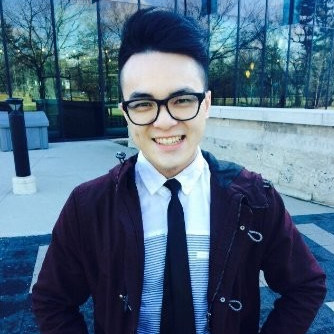
\includegraphics[width=\linewidth]{resources/image.jpeg}	%trimming relative to image size

%---------------------------------------------------------------------------------------
%	META SKILLS
%----------------------------------------------------------------------------------------
	\fcolorbox{white}{white}{\begin{minipage}[c][1.5cm][c]{1\mpwidth}
		\LARGE{\textbf{\textcolor{maincol}{Dominic Fung}}} \\[2pt]
		\normalsize{ \textcolor{maincol} {Bioinformatics and Statistics (BSc.)} }
\end{minipage}} \\
\icontext{CaretRight}{12}{Mississauga ON. Canada}{black}\\[6pt]


\cvsection{Skills}

\cvskill{Full stack development} {5+ yrs.} {1} \\[-2pt]

\cvskill{Cloud computing/ \newline Serverless technology} {3+ yrs.} {0.6} \\[-2pt]

\cvskill{Web dev. \& design} {4+ yrs.} {0.8} \\[-2pt]

\cvskill{App (IOS/Android) \newline development} {2+ yrs.} {0.4} \\[-2pt]

\cvskill{Big data/ \newline Data science} {2+ yrs.} {0.45} \\[-2pt]

\cvskill{Distributed ledger \newline technology} {1+ yrs.} {0.2} \\[-2pt]

\cvsection{Frameworks \& \newline Technologies}

\cvskill{Typescript \& Javascript} {4+ yrs.} {1} \\[-2pt]

\cvskill{Reactjs \& React-Native} {4+ yrs.} {0.92} \\[-2pt]

\cvskill{AWS serverless} {3+ yrs.} {0.9} \\[-2pt]

\cvskill{Python \& Tensorflow} {2+ yrs.} {0.5} \\[-2pt]

\cvskill{AWS Sagemaker} {2+ yrs.} {0.5} \\[-2pt]

\cvskill{Java/ Kotlin/ Swift} {1+ yrs.} {0.2} \\[-2pt]

\newpage
%---------------------------------------------------------------------------------------
%	EDUCATION
%----------------------------------------------------------------------------------------
\cvsection{Education}

\cvmetaevent
{2011 - 2016}
{Bioinformatics (BSc.) and \newline Minor Statistics}
{University of Toronto Mississauga}

% \cvmetaevent
% {XX/XXXX - XX/XXXX}
% {A-Level}
% {High School Rick Hanson}
% {\textit{Field 1 • Field 2 • Field 3 • Field 4 • Field 5}.}


\cvsection{Interests}

\icontext{CaretRight}{12}{Playing Music}{black}\\[6pt]
\icontext{CaretRight}{12}{Snowboarding}{black}\\[6pt]
\icontext{CaretRight}{12}{All things Marvel}{black}\\[6pt]




\cvsection{Contact}

\icontext{MapMarker}{16}{1406 Pickwick Dr. \\Mississauga ON. L5V 1V7}{black}\\[6pt]
\icontext{MobilePhone}{16}{+1 647 622 7764}{black}\\[6pt]
\iconemail{Envelope}{16}{dominic.fung@icloud.com}{dominic.fung@icloud.com}{black}\\[6pt]
\iconhref{Home}{16}{http://dom-fung.com}{http://dom-fung.com}{black}\\[6pt]
\iconhref{Github}{16}{github.com/DominicFung}{https://github.com/DominicFung}{black}\\[6pt]

	
%\cvqrcode{0.3}

\end{leftcolumn}
\begin{rightcolumn}
%---------------------------------------------------------------------------------------
%	TITLE  HEADER
%----------------------------------------------------------------------------------------


%---------------------------------------------------------------------------------------
%	PROFILE
%----------------------------------------------------------------------------------------
\cvsection{Biography}
\vspace{4pt}

\cvtext{
  Dominic is from Mississauga, Ontario where he works as a full-stack developer at Romet Limited. 
  Dom has 5 years of experience as a software developer with a focus on full-stack Javascript \& Typescript app development hosted on AWS.
  He's also dabbled in AI and blockchain technologies using Tensorflow and smart contracts on NEO respectively. 
  In his spare time, Dom plays acoustic renditions of 2000s punk-rock songs on his guitar and listens to Millennial Investing by The Investors's Podcast Network.
}


%---------------------------------------------------------------------------------------
%	WORK EXPERIENCE
%----------------------------------------------------------------------------------------

\vspace{14pt}
\cvsection{Work Experience}
\vspace{4pt}

\cvevent
{June 2021 - Today}
	{Full-Stack Developer | Romet Limited}
	{Research \& Development}
	{
    Worked on Android and iOS native apps for gas meter field technicians via Java/Swift with REST calls to AWS using API Gateway and lambda micro-services.
    Maintained our cloud infrastructure using CloudFormation and the serverless framework. Implemented multi-tiered deployment (test and production environments) with 
    CI/CD features via CodeCommit, CodeBuild, CodePipeline and CodeDeploy.\\[6pt]
    Augmented and implemented new features on the current data-portal built with Typescript React using GraphQL via AWS Amplify/Appsync talking to DynamoDB and RDS (Postgres).
    Worked on IoT Core and IoT Rules for data ingestion and device commission/decommission. 
    Used React-Native to build prototype Android/iOS/Desktop apps to communicate directly with meters using serial communication (RS232).
  }
	\vfill\null

\cvevent
{May 2017 - June 2021}
	{Technical Specialist | BMO}
	{RPA, Data \& AI - SmartCore}
	{
  Helped deploy multiple Workfusion and UiPath (robotic process automation, RPA) platforms on premise and in private cloud.
  Wrote multiple reusable Java libraries (ie. DB connectors, SMTP/IMAP) shared across projects.
  Built a video streaming platform using Reactjs, Videojs and RTMP to monitor automation in real-time.
  Integrated authentication and security via Active Director \& Cyberark. 
  %Created dashboards via PowerBI, reporting on server status, platform capacity and tracking in-flight automation projects.
  }
	\vfill\null

\cvevent
{Jan 2017 - May 2019}
	{IT Consultant | FDM Group}
	{Toronto, GTA}
	{Focused on helping customers build Java applications using relational DB backends (PostgreSQL, MySQL). 
  We utilized Spring Boot and the MVC design patterns.}
	\vfill\null
	

\cvsection{Projects}
\vspace{4pt}
	
\cvproject
	{Oslyn.io | Your digital bandmate}
	{Android \& IOS App, Artificial intelligence AI}
	{Oslyn is an app that listens to you play and accompanies you in real-time with a wide selection of pads, synths, and sounds. \\[6pt]
  As a data scientist, I used Tensorflow and AWS Sagemaker to train multiple model architectures (ie. Feed Forward, Recurrent Neural Net, etc.) 
  utilizing 400+ labelled songs and pretraining on web scraped audio data. \\[6pt]
  As a developer, I used AWS Amplify \& Cognito to authenticate and connect to our cloud infrastructure.
  DynamoDB \& AWS Appsync (graphQL) to store and fetch user data. S3 to store audio and AI model binaries. 
  I used React-Native + Java \& Swift deployed on the Play Store and App Store for Android and IOS respectively. \\[5pt]
  \iconhref{Link}{16}{https://oslyn.io}{https://oslyn.io/}{black} \\[1pt]} 
  {resources/oslyn.png}
	\vfill\null
  

\cvproject
	{Nodis.io | Get Noticed}
	{Webapp and Blockchain}
	{Nodis’ goal is to help small businesses around the world to get noticed by local communities. 
  Nodis Challenge is our fun and interactive way to reach that goal. 
  Nodis is a cryptocurrency, built on the NEO blockchain using Reactjs and MongoDB hosted on AWS EC2. 
  I also helped test the smart contract on the NEO test network using Python. \\[6pt]
  \iconhref{Link}{16}{https://nodis.io}{https://nodis.io/}{black} \\
  \iconhref{Github}{16}{https://github.com/nodis-io}{https://github.com/nodis-io}{black}\\[1pt]
  }
  {resources/nodis.jpeg}
	\vfill\null


\cvproject
	{One Chanhs Co. | Bridal store}
	{Serverless React store}
	{Built with React and AWS Appsync. Stripe API for monetization. \newline
  Used tailwind.css to allow my client greater design customizability. \\[6pt]
  \iconhref{Link}{16}{https://onechanhs.ca}{https://onechanhs.ca/}{black} \\
  \iconhref{Github}{16}{https://github.com/DominicFung/onechanhs}{https://github.com/DominicFung/onechanhs}{black}\\[6pt]
  }
  {resources/onechanhs.png}
	\vfill\null


\cvproject
	{Logistical.ly}
	{Desktop app via React-Electron}
	{Windows desktop app built with Typescript, React and Electron to 
  help a client find the lowest courier cost given a list of destinations and 
  courier services. \\[6pt]
  \iconhref{Github}{16}{https://github.com/DominicFung/logistical.ly}{https://github.com/DominicFung/logistical.ly}{black}\\[6pt]
  }
  {resources/logistically.png}
	\vfill\null


\cvsection{Certifications}

\cvcertification
  {Amazon Web Services Solutions Architect Associate}
  {Amazon Web Services (AWS)}
  {HDW98122JFRQQBGT}
  {resources/aws-cert.jpeg}
  \vfill\null

\cvcertification
  {SAS Certified Advanced Programmer for SAS 9}
  {SAS Institute}
  {AP019093v9}
  {resources/sas-cert.jpeg}
  \vfill\null

\cvcertification
  {MTA: Database Fundamentals - Certified 2016}
  {Microsoft}
  {13090778}
  {resources/microsoft-cert.jpeg}
  \vfill\null

% hofixes to create fake-space to ensure the whole height is used
\mbox{}
\vfill
\mbox{}
% \vfill
% \mbox{}
% \vfill
% \mbox{}
% \vfill
% \mbox{}
% \vfill
% \mbox{}
% \vfill
% \mbox{}

\end{rightcolumn}
\end{paracol}

\mbox{}
\vfill
\mbox{}

\today     \hspace{1cm}   \hrulefill

\hspace*{62mm}\phantom{ \today } Dominic Fung




\end{document}